\documentclass[14pt]{extbook}
\usepackage{multicol, enumerate, enumitem, hyperref, color, soul, setspace, parskip, fancyhdr} %General Packages
\usepackage{amssymb, amsthm, amsmath, latexsym, units, mathtools} %Math Packages
\everymath{\displaystyle} %All math in Display Style
% Packages with additional options
\usepackage[headsep=0.5cm,headheight=12pt, left=1 in,right= 1 in,top= 1 in,bottom= 1 in]{geometry}
\usepackage[usenames,dvipsnames]{xcolor}
\usepackage{dashrule}  % Package to use the command below to create lines between items
\newcommand{\litem}[1]{\item#1\hspace*{-1cm}\rule{\textwidth}{0.4pt}}
\pagestyle{fancy}
\lhead{Progress Quiz 9}
\chead{}
\rhead{Version ALL}
\lfoot{9541-5764}
\cfoot{}
\rfoot{Summer C 2021}
\begin{document}

\begin{enumerate}
\litem{
Choose the equation of the function graphed below.
\begin{center}
    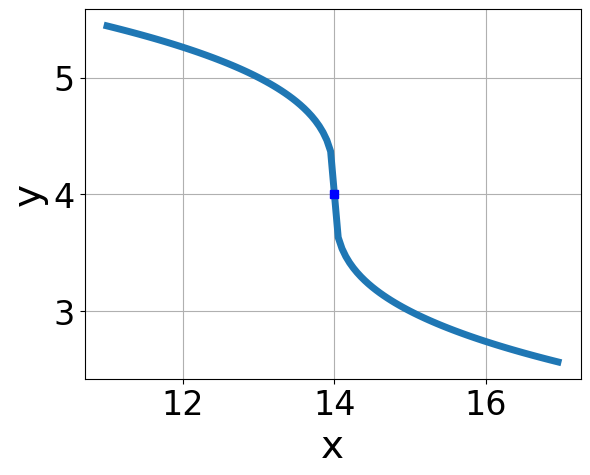
\includegraphics[width=0.5\textwidth]{../Figures/radicalGraphToEquationA.png}
\end{center}
\begin{enumerate}[label=\Alph*.]
\item \( f(x) = - \sqrt{x + 14} + 4 \)
\item \( f(x) = \sqrt{x + 14} + 4 \)
\item \( f(x) = - \sqrt{x - 14} + 4 \)
\item \( f(x) = \sqrt{x - 14} + 4 \)
\item \( \text{None of the above} \)

\end{enumerate} }
\litem{
Choose the equation of the function graphed below.
\begin{center}
    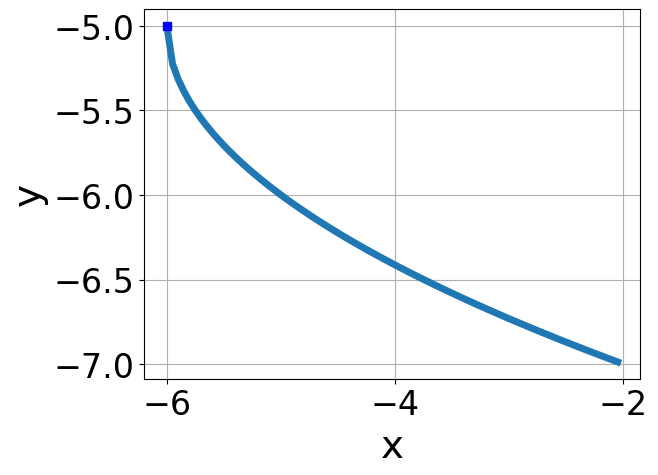
\includegraphics[width=0.5\textwidth]{../Figures/radicalGraphToEquationCopyA.png}
\end{center}
\begin{enumerate}[label=\Alph*.]
\item \( f(x) = - \sqrt{x + 6} - 5 \)
\item \( f(x) = - \sqrt{x - 6} - 5 \)
\item \( f(x) = \sqrt{x + 6} - 5 \)
\item \( f(x) = \sqrt{x - 6} - 5 \)
\item \( \text{None of the above} \)

\end{enumerate} }
\litem{
Solve the radical equation below. Then, choose the interval(s) that the solution(s) belongs to.\[ \sqrt{21 x^2 + 36} - \sqrt{-55 x} = 0 \]\begin{enumerate}[label=\Alph*.]
\item \( x_1 \in [1.26, 1.43] \text{ and } x_2 \in [-0.67,6.33] \)
\item \( \text{All solutions lead to invalid or complex values in the equation.} \)
\item \( x \in [-1.35,-1.29] \)
\item \( x \in [-1.29,-1.27] \)
\item \( x_1 \in [-1.35, -1.29] \text{ and } x_2 \in [-4.29,-0.29] \)

\end{enumerate} }
\litem{
Solve the radical equation below. Then, choose the interval(s) that the solution(s) belongs to.\[ \sqrt{-3 x + 2} - \sqrt{9 x - 8} = 0 \]\begin{enumerate}[label=\Alph*.]
\item \( x_1 \in [0.6, 0.71] \text{ and } x_2 \in [0.81,0.86] \)
\item \( x_1 \in [0.6, 0.71] \text{ and } x_2 \in [0.86,0.95] \)
\item \( x \in [0.7,0.94] \)
\item \( x \in [-0.52,-0.37] \)
\item \( \text{All solutions lead to invalid or complex values in the equation.} \)

\end{enumerate} }
\litem{
What is the domain of the function below?\[ f(x) = \sqrt[7]{-9 x - 8} \]\begin{enumerate}[label=\Alph*.]
\item \( \text{The domain is } (-\infty, a], \text{   where } a \in [-1.58, -0.89] \)
\item \( \text{The domain is } [a, \infty), \text{   where } a \in [-1.41, -0.9] \)
\item \( \text{The domain is } [a, \infty), \text{   where } a \in [-1.07, -0.53] \)
\item \( (-\infty, \infty) \)
\item \( \text{The domain is } (-\infty, a], \text{   where } a \in [-1.12, -0.1] \)

\end{enumerate} }
\litem{
Choose the graph of the equation below.\[ f(x) = \sqrt{x - 6} + 6 \]\begin{enumerate}[label=\Alph*.]
\begin{multicols}{2}\item 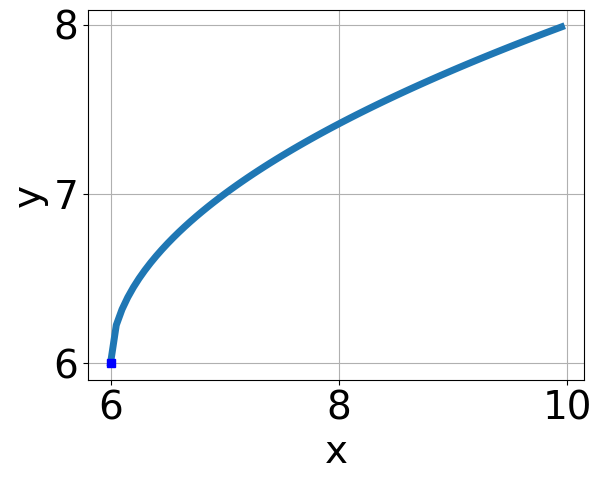
\includegraphics[width = 0.3\textwidth]{../Figures/radicalEquationToGraphAA.png}\item 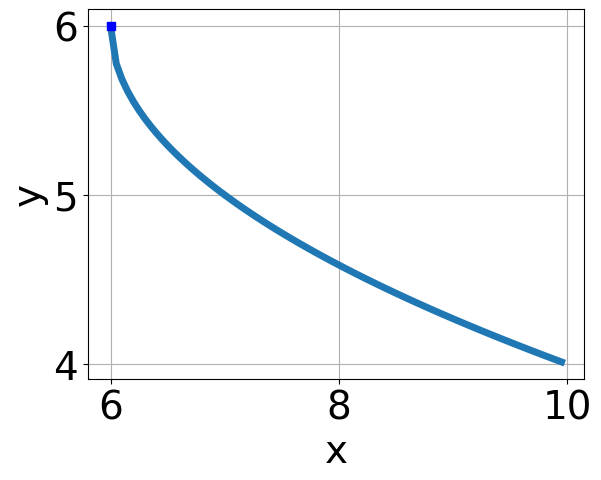
\includegraphics[width = 0.3\textwidth]{../Figures/radicalEquationToGraphBA.png}\item 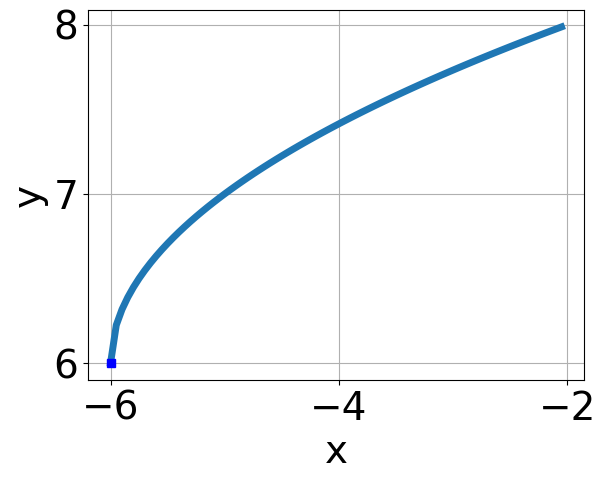
\includegraphics[width = 0.3\textwidth]{../Figures/radicalEquationToGraphCA.png}\item 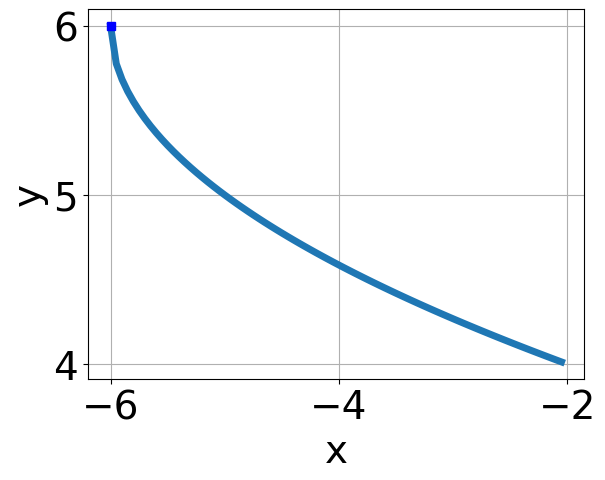
\includegraphics[width = 0.3\textwidth]{../Figures/radicalEquationToGraphDA.png}\end{multicols}\item None of the above.
\end{enumerate} }
\litem{
What is the domain of the function below?\[ f(x) = \sqrt[7]{8 x - 9} \]\begin{enumerate}[label=\Alph*.]
\item \( (-\infty, \infty) \)
\item \( \text{The domain is } (-\infty, a], \text{   where } a \in [1.03, 2.09] \)
\item \( \text{The domain is } (-\infty, a], \text{   where } a \in [0.88, 0.92] \)
\item \( \text{The domain is } [a, \infty), \text{   where } a \in [0.86, 1.12] \)
\item \( \text{The domain is } [a, \infty), \text{   where } a \in [1.11, 1.38] \)

\end{enumerate} }
\litem{
Solve the radical equation below. Then, choose the interval(s) that the solution(s) belongs to.\[ \sqrt{18 x^2 + 40} - \sqrt{-61 x} = 0 \]\begin{enumerate}[label=\Alph*.]
\item \( x_1 \in [-3.63, -1.99] \text{ and } x_2 \in [-3.89,0.11] \)
\item \( x \in [-1.96,-0.45] \)
\item \( x_1 \in [-0.22, 1.61] \text{ and } x_2 \in [2.5,3.5] \)
\item \( \text{All solutions lead to invalid or complex values in the equation.} \)
\item \( x \in [-3.63,-1.99] \)

\end{enumerate} }
\litem{
Choose the graph of the equation below.\[ f(x) = \sqrt[3]{x + 12} - 3 \]\begin{enumerate}[label=\Alph*.]
\begin{multicols}{2}\item 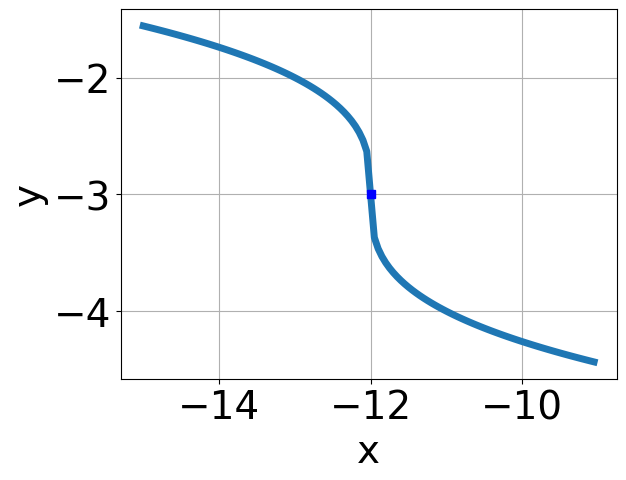
\includegraphics[width = 0.3\textwidth]{../Figures/radicalEquationToGraphCopyAA.png}\item 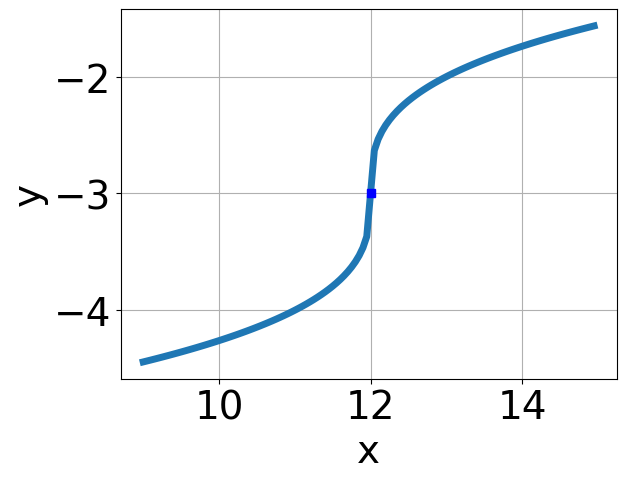
\includegraphics[width = 0.3\textwidth]{../Figures/radicalEquationToGraphCopyBA.png}\item 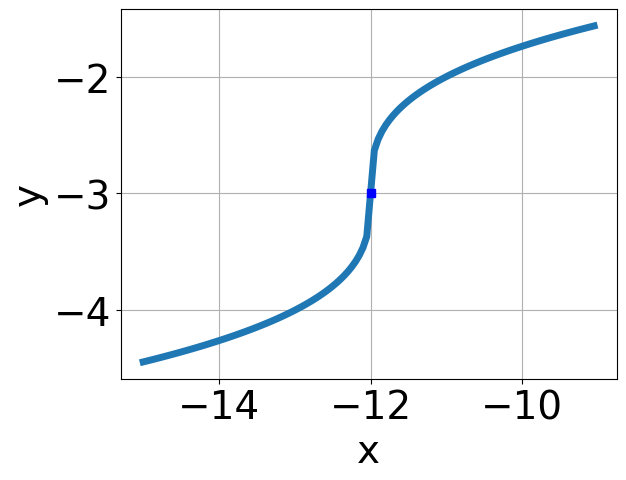
\includegraphics[width = 0.3\textwidth]{../Figures/radicalEquationToGraphCopyCA.png}\item 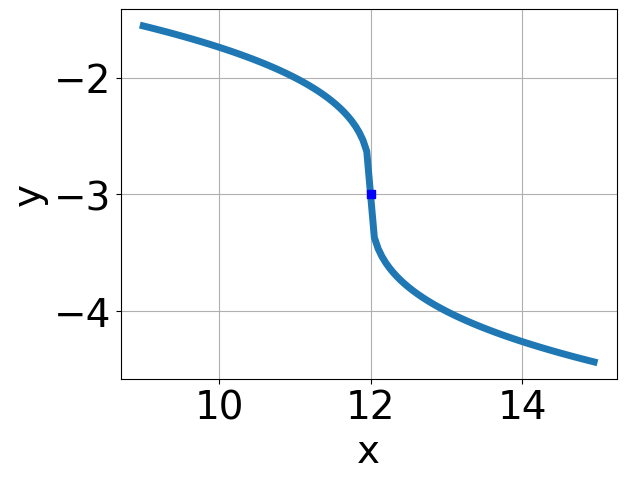
\includegraphics[width = 0.3\textwidth]{../Figures/radicalEquationToGraphCopyDA.png}\end{multicols}\item None of the above.
\end{enumerate} }
\litem{
Solve the radical equation below. Then, choose the interval(s) that the solution(s) belongs to.\[ \sqrt{7 x + 5} - \sqrt{-3 x - 9} = 0 \]\begin{enumerate}[label=\Alph*.]
\item \( x_1 \in [-3.4, -2.8] \text{ and } x_2 \in [-2.71,4.29] \)
\item \( x_1 \in [-1.6, -0.3] \text{ and } x_2 \in [-2.71,4.29] \)
\item \( x \in [-1.6,-0.3] \)
\item \( \text{All solutions lead to invalid or complex values in the equation.} \)
\item \( x \in [-1.1,0.5] \)

\end{enumerate} }
\litem{
Choose the equation of the function graphed below.
\begin{center}
    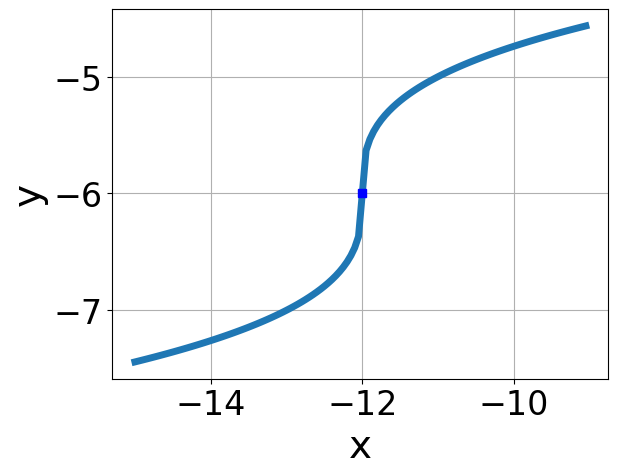
\includegraphics[width=0.5\textwidth]{../Figures/radicalGraphToEquationB.png}
\end{center}
\begin{enumerate}[label=\Alph*.]
\item \( f(x) = \sqrt{x + 12} - 6 \)
\item \( f(x) = \sqrt{x - 12} - 6 \)
\item \( f(x) = - \sqrt{x - 12} - 6 \)
\item \( f(x) = - \sqrt{x + 12} - 6 \)
\item \( \text{None of the above} \)

\end{enumerate} }
\litem{
Choose the equation of the function graphed below.
\begin{center}
    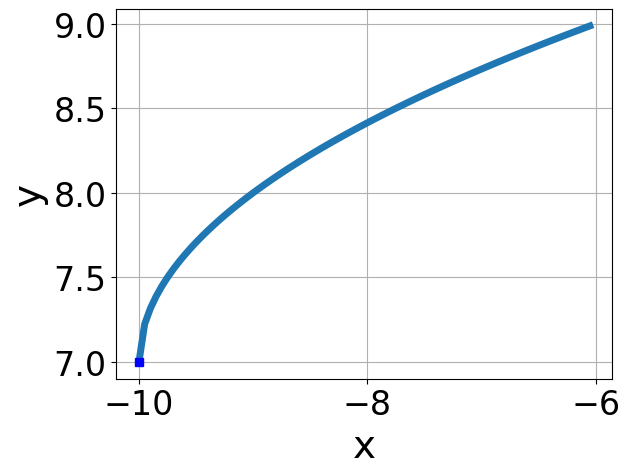
\includegraphics[width=0.5\textwidth]{../Figures/radicalGraphToEquationCopyB.png}
\end{center}
\begin{enumerate}[label=\Alph*.]
\item \( f(x) = - \sqrt{x - 10} + 7 \)
\item \( f(x) = \sqrt{x - 10} + 7 \)
\item \( f(x) = \sqrt{x + 10} + 7 \)
\item \( f(x) = - \sqrt{x + 10} + 7 \)
\item \( \text{None of the above} \)

\end{enumerate} }
\litem{
Solve the radical equation below. Then, choose the interval(s) that the solution(s) belongs to.\[ \sqrt{14 x^2 - 12} - \sqrt{-13 x} = 0 \]\begin{enumerate}[label=\Alph*.]
\item \( x \in [-2.71,-0.05] \)
\item \( x \in [-0.03,1.04] \)
\item \( x_1 \in [-0.03, 1.04] \text{ and } x_2 \in [1.18,2.2] \)
\item \( \text{All solutions lead to invalid or complex values in the equation.} \)
\item \( x_1 \in [-2.71, -0.05] \text{ and } x_2 \in [-0.34,0.79] \)

\end{enumerate} }
\litem{
Solve the radical equation below. Then, choose the interval(s) that the solution(s) belongs to.\[ \sqrt{5 x - 8} - \sqrt{8 x - 5} = 0 \]\begin{enumerate}[label=\Alph*.]
\item \( x \in [-3,0] \)
\item \( \text{All solutions lead to invalid or complex values in the equation.} \)
\item \( x_1 \in [-0.38, 5.62] \text{ and } x_2 \in [0.6,3.6] \)
\item \( x \in [-7.33,-1.33] \)
\item \( x_1 \in [-3, 0] \text{ and } x_2 \in [0.6,3.6] \)

\end{enumerate} }
\litem{
What is the domain of the function below?\[ f(x) = \sqrt[4]{-5 x + 8} \]\begin{enumerate}[label=\Alph*.]
\item \( (-\infty, \infty) \)
\item \( [a, \infty), \text{where } a \in [1.46, 1.79] \)
\item \( [a, \infty), \text{where } a \in [0.35, 1.05] \)
\item \( (-\infty, a], \text{where } a \in [0.2, 0.8] \)
\item \( (-\infty, a], \text{ where } a \in [1.2, 3] \)

\end{enumerate} }
\litem{
Choose the graph of the equation below.\[ f(x) = - \sqrt[3]{x - 8} + 4 \]\begin{enumerate}[label=\Alph*.]
\begin{multicols}{2}\item 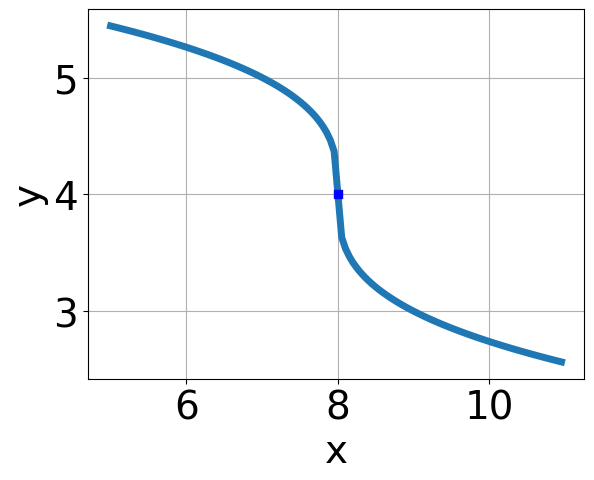
\includegraphics[width = 0.3\textwidth]{../Figures/radicalEquationToGraphAB.png}\item 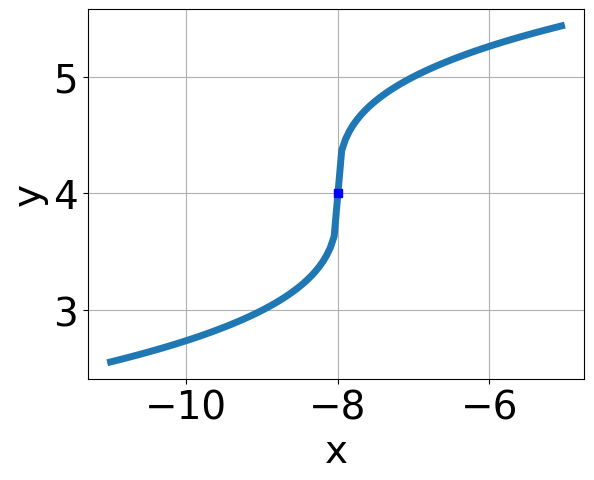
\includegraphics[width = 0.3\textwidth]{../Figures/radicalEquationToGraphBB.png}\item 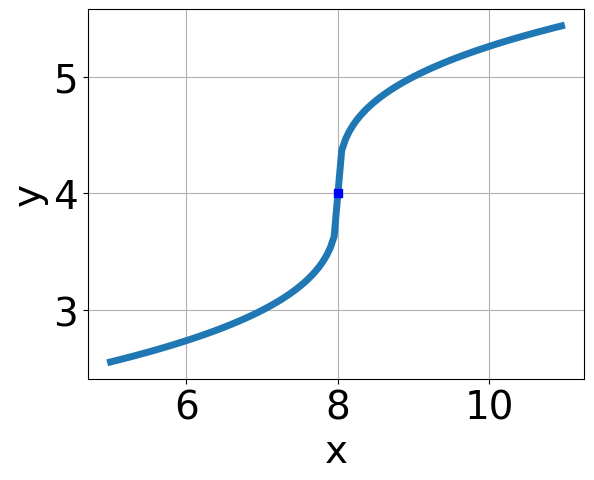
\includegraphics[width = 0.3\textwidth]{../Figures/radicalEquationToGraphCB.png}\item 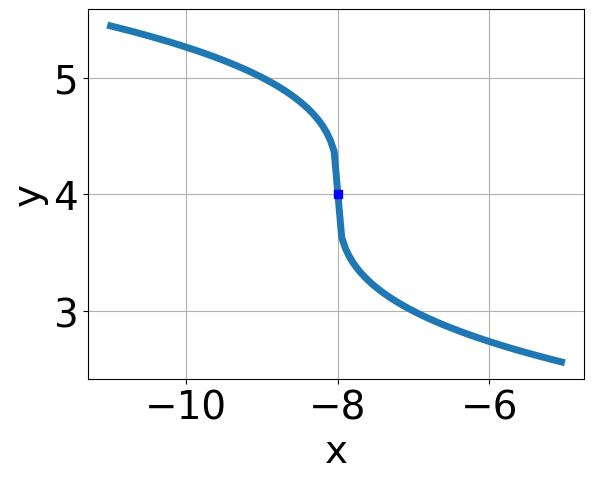
\includegraphics[width = 0.3\textwidth]{../Figures/radicalEquationToGraphDB.png}\end{multicols}\item None of the above.
\end{enumerate} }
\litem{
What is the domain of the function below?\[ f(x) = \sqrt[7]{8 x - 9} \]\begin{enumerate}[label=\Alph*.]
\item \( (-\infty, \infty) \)
\item \( \text{The domain is } [a, \infty), \text{   where } a \in [0.92, 1.31] \)
\item \( \text{The domain is } (-\infty, a], \text{   where } a \in [0.71, 1.01] \)
\item \( \text{The domain is } (-\infty, a], \text{   where } a \in [1.03, 1.25] \)
\item \( \text{The domain is } [a, \infty), \text{   where } a \in [0.86, 0.94] \)

\end{enumerate} }
\litem{
Solve the radical equation below. Then, choose the interval(s) that the solution(s) belongs to.\[ \sqrt{9 x^2 + 6} - \sqrt{15 x} = 0 \]\begin{enumerate}[label=\Alph*.]
\item \( x \in [0.2,0.91] \)
\item \( x_1 \in [0.2, 0.91] \text{ and } x_2 \in [0.3,4.3] \)
\item \( x \in [0.98,1.04] \)
\item \( x_1 \in [-1.07, -0.43] \text{ and } x_2 \in [-2.5,0.1] \)
\item \( \text{All solutions lead to invalid or complex values in the equation.} \)

\end{enumerate} }
\litem{
Choose the graph of the equation below.\[ f(x) = \sqrt{x - 10} + 4 \]\begin{enumerate}[label=\Alph*.]
\begin{multicols}{2}\item 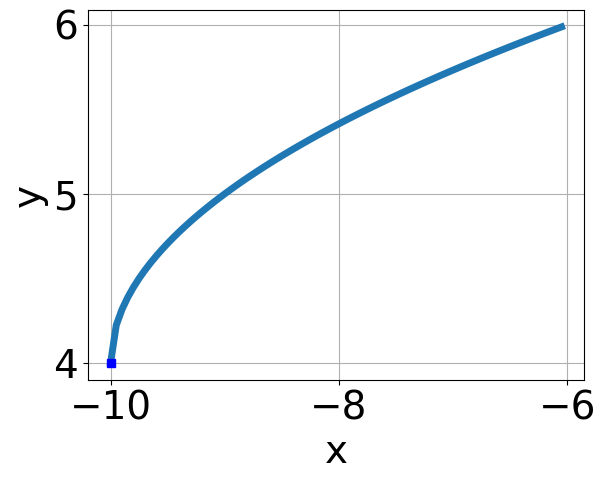
\includegraphics[width = 0.3\textwidth]{../Figures/radicalEquationToGraphCopyAB.png}\item 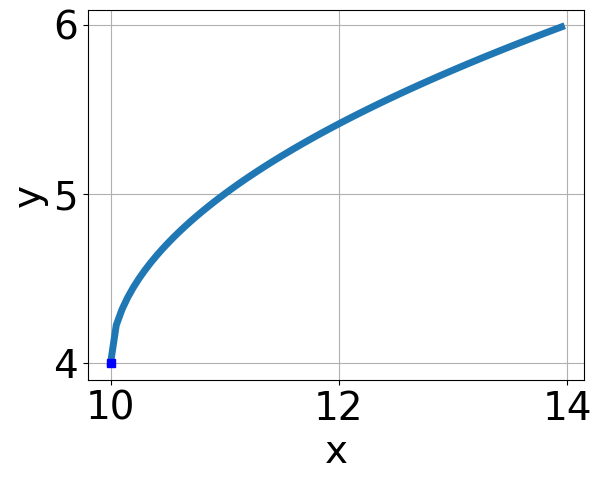
\includegraphics[width = 0.3\textwidth]{../Figures/radicalEquationToGraphCopyBB.png}\item 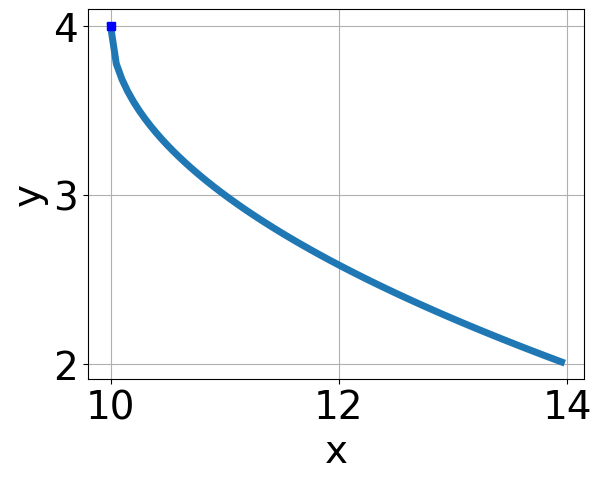
\includegraphics[width = 0.3\textwidth]{../Figures/radicalEquationToGraphCopyCB.png}\item 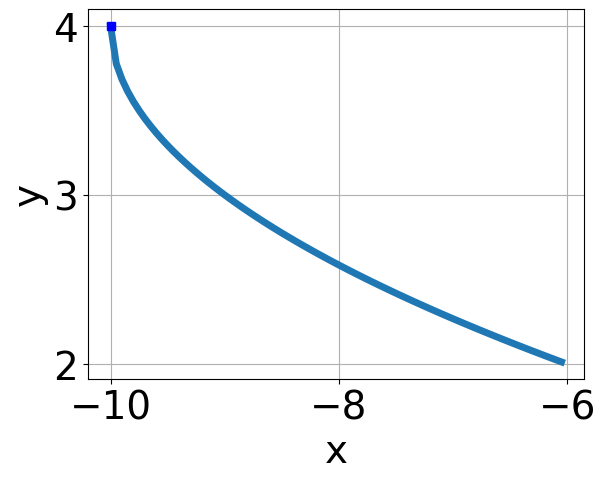
\includegraphics[width = 0.3\textwidth]{../Figures/radicalEquationToGraphCopyDB.png}\end{multicols}\item None of the above.
\end{enumerate} }
\litem{
Solve the radical equation below. Then, choose the interval(s) that the solution(s) belongs to.\[ \sqrt{8 x + 8} - \sqrt{-2 x + 7} = 0 \]\begin{enumerate}[label=\Alph*.]
\item \( x \in [-2.14,-1.24] \)
\item \( x \in [-0.76,0] \)
\item \( x_1 \in [-1.48, -0.65] \text{ and } x_2 \in [1.5,6.5] \)
\item \( \text{All solutions lead to invalid or complex values in the equation.} \)
\item \( x_1 \in [-1.48, -0.65] \text{ and } x_2 \in [-0.1,1.9] \)

\end{enumerate} }
\litem{
Choose the equation of the function graphed below.
\begin{center}
    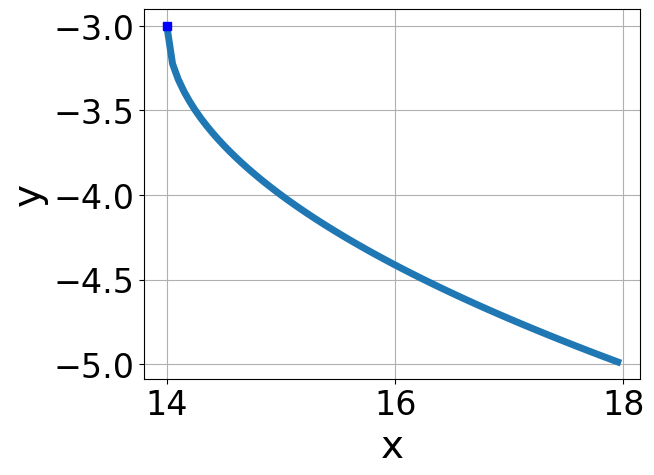
\includegraphics[width=0.5\textwidth]{../Figures/radicalGraphToEquationC.png}
\end{center}
\begin{enumerate}[label=\Alph*.]
\item \( f(x) = - \sqrt[3]{x + 14} - 3 \)
\item \( f(x) = \sqrt[3]{x - 14} - 3 \)
\item \( f(x) = - \sqrt[3]{x - 14} - 3 \)
\item \( f(x) = \sqrt[3]{x + 14} - 3 \)
\item \( \text{None of the above} \)

\end{enumerate} }
\litem{
Choose the equation of the function graphed below.
\begin{center}
    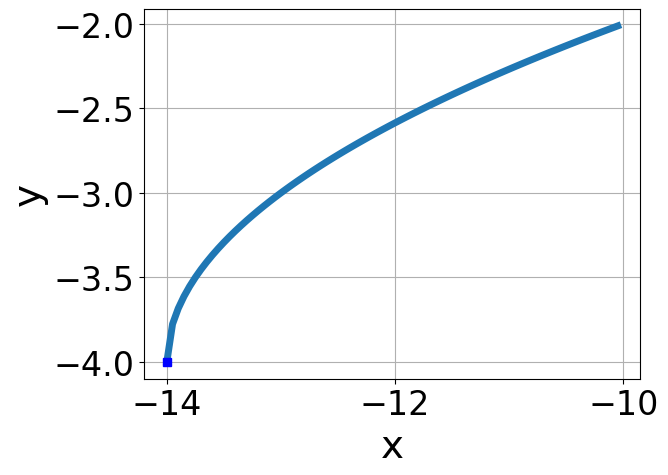
\includegraphics[width=0.5\textwidth]{../Figures/radicalGraphToEquationCopyC.png}
\end{center}
\begin{enumerate}[label=\Alph*.]
\item \( f(x) = - \sqrt[3]{x + 14} - 4 \)
\item \( f(x) = - \sqrt[3]{x - 14} - 4 \)
\item \( f(x) = \sqrt[3]{x + 14} - 4 \)
\item \( f(x) = \sqrt[3]{x - 14} - 4 \)
\item \( \text{None of the above} \)

\end{enumerate} }
\litem{
Solve the radical equation below. Then, choose the interval(s) that the solution(s) belongs to.\[ \sqrt{-15 x^2 + 63} - \sqrt{24 x} = 0 \]\begin{enumerate}[label=\Alph*.]
\item \( x_1 \in [1.4, 4.4] \text{ and } x_2 \in [1.6,3.4] \)
\item \( x \in [-3,0] \)
\item \( x_1 \in [-3, 0] \text{ and } x_2 \in [-0.5,2.2] \)
\item \( \text{All solutions lead to invalid or complex values in the equation.} \)
\item \( x \in [1.4,4.4] \)

\end{enumerate} }
\litem{
Solve the radical equation below. Then, choose the interval(s) that the solution(s) belongs to.\[ \sqrt{-5 x + 2} - \sqrt{8 x + 8} = 0 \]\begin{enumerate}[label=\Alph*.]
\item \( x_1 \in [-0.55, -0.31] \text{ and } x_2 \in [0.4,7.4] \)
\item \( x \in [0,1.15] \)
\item \( \text{All solutions lead to invalid or complex values in the equation.} \)
\item \( x_1 \in [-1.33, -0.99] \text{ and } x_2 \in [0.4,7.4] \)
\item \( x \in [-0.55,-0.31] \)

\end{enumerate} }
\litem{
What is the domain of the function below?\[ f(x) = \sqrt[5]{-6 x + 7} \]\begin{enumerate}[label=\Alph*.]
\item \( (-\infty, \infty) \)
\item \( \text{The domain is } (-\infty, a], \text{   where } a \in [1.02, 1.48] \)
\item \( \text{The domain is } (-\infty, a], \text{   where } a \in [0.74, 0.96] \)
\item \( \text{The domain is } [a, \infty), \text{   where } a \in [0.21, 1.13] \)
\item \( \text{The domain is } [a, \infty), \text{   where } a \in [1.03, 1.43] \)

\end{enumerate} }
\litem{
Choose the graph of the equation below.\[ f(x) = \sqrt[3]{x + 12} - 7 \]\begin{enumerate}[label=\Alph*.]
\begin{multicols}{2}\item 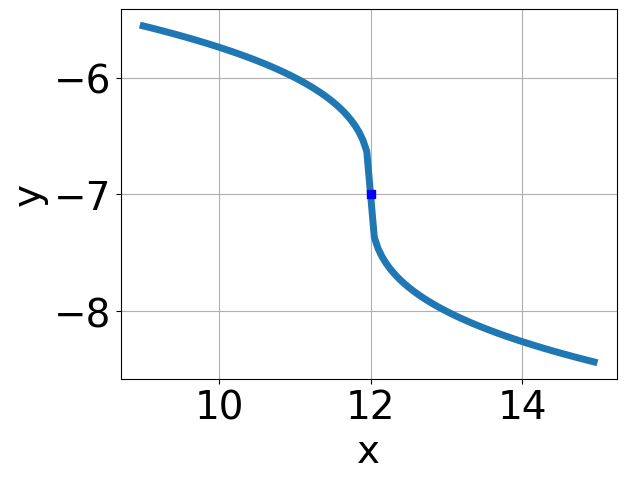
\includegraphics[width = 0.3\textwidth]{../Figures/radicalEquationToGraphAC.png}\item 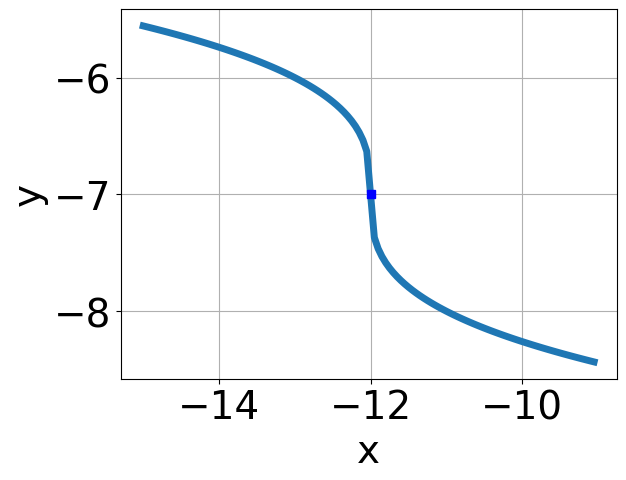
\includegraphics[width = 0.3\textwidth]{../Figures/radicalEquationToGraphBC.png}\item 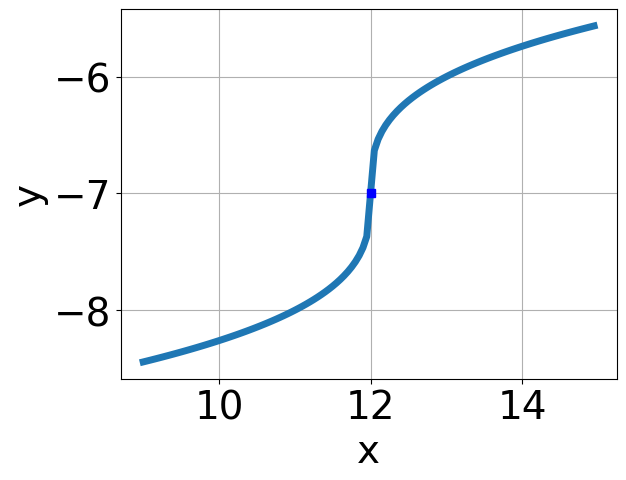
\includegraphics[width = 0.3\textwidth]{../Figures/radicalEquationToGraphCC.png}\item 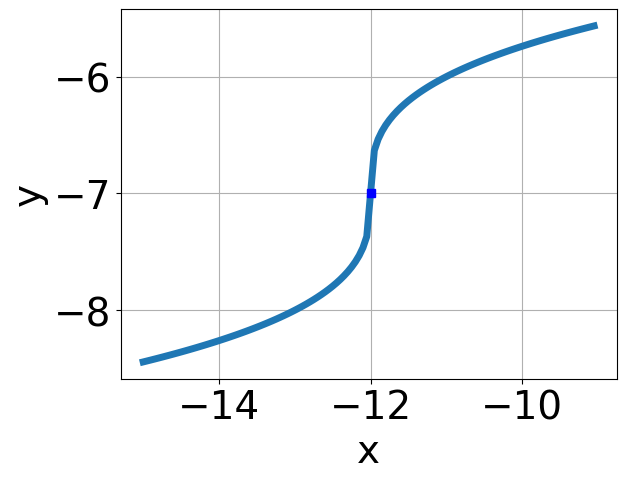
\includegraphics[width = 0.3\textwidth]{../Figures/radicalEquationToGraphDC.png}\end{multicols}\item None of the above.
\end{enumerate} }
\litem{
What is the domain of the function below?\[ f(x) = \sqrt[7]{-9 x + 3} \]\begin{enumerate}[label=\Alph*.]
\item \( \text{The domain is } [a, \infty), \text{   where } a \in [2, 5] \)
\item \( \text{The domain is } (-\infty, a], \text{   where } a \in [0.3, 1.1] \)
\item \( \text{The domain is } (-\infty, a], \text{   where } a \in [2.8, 4.1] \)
\item \( \text{The domain is } [a, \infty), \text{   where } a \in [-5.67, 2.33] \)
\item \( (-\infty, \infty) \)

\end{enumerate} }
\litem{
Solve the radical equation below. Then, choose the interval(s) that the solution(s) belongs to.\[ \sqrt{-36 x^2 - 10} - \sqrt{-42 x} = 0 \]\begin{enumerate}[label=\Alph*.]
\item \( x_1 \in [0.15, 0.65] \text{ and } x_2 \in [0.6,1.6] \)
\item \( x \in [0.7,0.85] \)
\item \( x \in [0.15,0.65] \)
\item \( \text{All solutions lead to invalid or complex values in the equation.} \)
\item \( x_1 \in [-0.47, -0.2] \text{ and } x_2 \in [-2.6,-0.7] \)

\end{enumerate} }
\litem{
Choose the graph of the equation below.\[ f(x) = \sqrt{x - 14} + 7 \]\begin{enumerate}[label=\Alph*.]
\begin{multicols}{2}\item 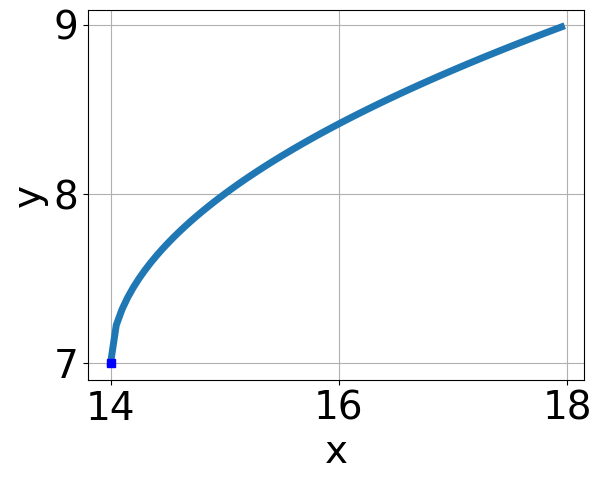
\includegraphics[width = 0.3\textwidth]{../Figures/radicalEquationToGraphCopyAC.png}\item 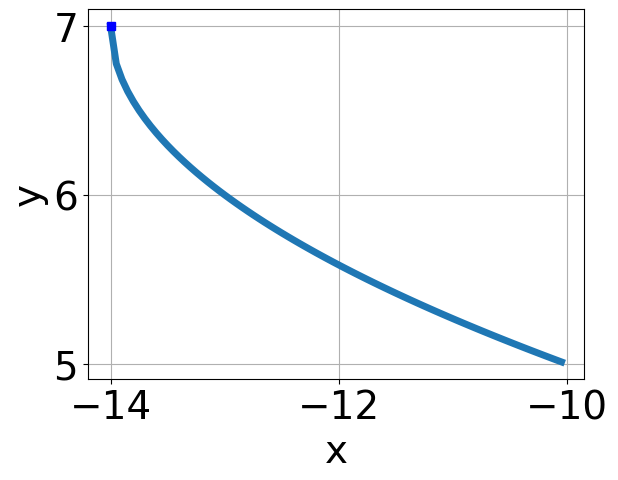
\includegraphics[width = 0.3\textwidth]{../Figures/radicalEquationToGraphCopyBC.png}\item 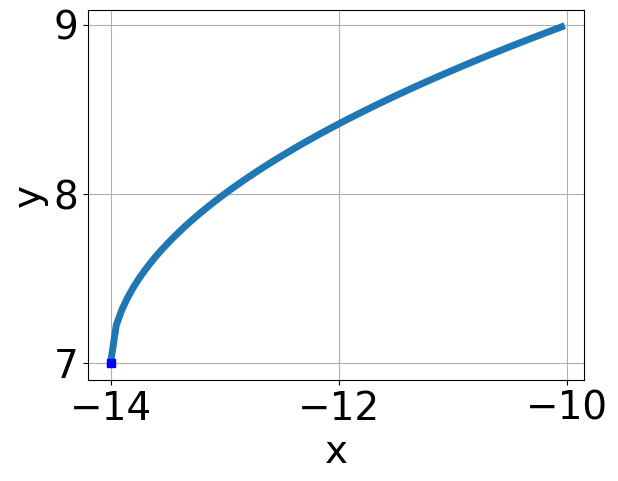
\includegraphics[width = 0.3\textwidth]{../Figures/radicalEquationToGraphCopyCC.png}\item 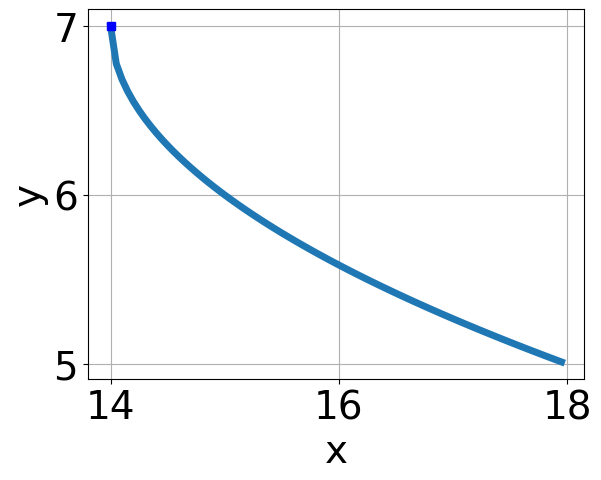
\includegraphics[width = 0.3\textwidth]{../Figures/radicalEquationToGraphCopyDC.png}\end{multicols}\item None of the above.
\end{enumerate} }
\litem{
Solve the radical equation below. Then, choose the interval(s) that the solution(s) belongs to.\[ \sqrt{9 x - 9} - \sqrt{-5 x - 3} = 0 \]\begin{enumerate}[label=\Alph*.]
\item \( x_1 \in [-0.87, 0.4] \text{ and } x_2 \in [1,5] \)
\item \( x \in [-0.11,0.48] \)
\item \( \text{All solutions lead to invalid or complex values in the equation.} \)
\item \( x \in [0.78,1.87] \)
\item \( x_1 \in [-0.11, 0.48] \text{ and } x_2 \in [1,5] \)

\end{enumerate} }
\end{enumerate}

\end{document}